\documentclass[conference]{IEEEtran}

\usepackage[utf8]{inputenc}
\usepackage[T1]{fontenc}
\usepackage{cite}
\usepackage{amsmath,amssymb}
\usepackage{graphicx}
\usepackage{booktabs}
\usepackage{multirow}
\usepackage{array}
\usepackage[table]{xcolor}
\usepackage{url}
\usepackage[hidelinks]{hyperref}

% figures live in the repository's figures/ folder; a local copy in report/figures/ also works
\graphicspath{{../figures/}{figures/}}

\newcommand{\best}[1]{\textbf{#1}}

\begin{document}

\title{Does Sentiment Help Catch a Liar?\\
Sentiment and Tone-Change Features for Deception Detection in \textit{Diplomacy}\\
{\large CS 415 Progress Report --- Group 7}}

\author{
\IEEEauthorblockN{Do\u{g}ukan Do\u{g}an}
\IEEEauthorblockA{Student ID: 31053}
\and
\IEEEauthorblockN{Pelin Durukan}
\IEEEauthorblockA{Student ID: 33993}
\and
\IEEEauthorblockN{Bet\"{u}l Eken}
\IEEEauthorblockA{Student ID: 34378}
}

\maketitle

% =====================================================================
\begin{abstract}
We study whether the sentiment of a message, and how that sentiment shifts relative to the sender's own earlier messages (\emph{tone change}), helps to detect lies in the \textit{Diplomacy} deception dataset of Peskov et al.\ (17{,}289 messages; 4--9\% lies). So far we have (i)~reproduced the majority and bag-of-words baselines of the original paper to within 0.3 macro F1; (ii)~scored every message with a lexicon-based (VADER) and a transformer-based (Twitter-RoBERTa) sentiment model and tested whether lies and truths differ in sentiment; (iii)~built 13 leakage-free tone-change features; (iv)~trained logistic regression models under leave-one-game-out cross-validation; and (v)~fine-tuned RoBERTa with conversational context and power features, with and without sentiment and tone-change features, over five random seeds. Lies and truths do differ in sentiment (H1), but only negligibly ($|r|<0.1$), and the difference is largely explained by the fact that lies are longer. A classifier using only sentiment and tone-change features beats the majority class (H2), but is weaker than one using message length alone. In the fine-tuned model, sentiment features lower lie F1 by 4.1 points on average (H3 not supported), while tone-change features then raise it by 5.5 points (H4 supported); the full model is not significantly better than the model with neither. Our best model, a five-seed ensemble of the full model, reaches 57.1 macro F1 and 20.6 lie F1 on the official test games. This nearly matches the best macro F1 of the original paper (57.2) but not its lie F1 (27.0), so it falls short of the success criteria set in our proposal.
\end{abstract}

\begin{IEEEkeywords}
deception detection, sentiment analysis, Diplomacy, RoBERTa, class imbalance, computational social science
\end{IEEEkeywords}

% =====================================================================
\section{Introduction}
\label{sec:intro}

\subsection{Problem}
Trust underlies most online conversations, and it can be betrayed through deception. Much of the work on detecting deception in text studies \emph{one-off} lies: a fake product review, a statement made on instruction in a lab, or a single testimony in court. In many real relationships, however, deception is \emph{strategic and sustained}: the same person mixes truthful and deceptive messages over a long conversation to reach a goal. The board game \textit{Diplomacy} is a natural testbed for this. Seven players negotiate alliances in private messages, and since nobody can win alone, every player must decide, message by message, whether to be honest. Peskov et al.~\cite{peskov2020takes} collected 12 such games in which every sender marked each message as truthful or a lie at the time of writing (the \textsc{Actual Lie} label), and every receiver marked whether they believed it (the \textsc{Suspected Lie} label).

Our task is to predict the sender's label: \emph{given a message and its conversational history, is it a lie?}

\subsection{Motivation}
Lie detection is hard for people and machines alike. Humans are barely better than chance at judging deception (54\% accuracy on average in a meta-analysis of 206 documents~\cite{bond2006accuracy}) and show a strong truth bias~\cite{levine1999veracity}. In \textit{Diplomacy} the receivers detect lies with a lie F1 of only 22.5~\cite{peskov2020takes}. The best model of Peskov et al., a hierarchical LSTM over the conversation with power features, reaches 57.2 macro F1 and 27.0 lie F1, so there is substantial room for improvement.

Sentiment is a promising and so far unused signal for this task. Psychology suggests that liars express emotion differently. Meta-analyses find more negative and less pleasant language in lies~\cite{depaulo2003cues,newman2003lying}, while studies of computer-mediated communication find that liars write \emph{more} words and more emotional words~\cite{hancock2008lying,zhou2004automating}. Closest to our setting, Niculae et al.~\cite{niculae2015harbingers} showed on \textit{Diplomacy} games that a coming betrayal is foreshadowed by \emph{sudden changes} in the betrayer's positive sentiment and politeness. This suggests that it is not only the sentiment of a message that matters but how it departs from the sender's usual tone. Peskov et al.'s models use words, conversational context and power, but no explicit sentiment or tone-change information.

\subsection{Research question and hypotheses}
\emph{Does the sentiment of a message, and in particular how it changes compared with the sender's earlier messages, help to detect whether that message is a lie?} Our proposal set four hypotheses:
\begin{itemize}
\item \textbf{H1}: the sentiment of lies differs from that of truthful messages ($p < 0.05$).
\item \textbf{H2}: a classifier using only sentiment and tone-change features beats the majority class (macro F1 $> 47.8$).
\item \textbf{H3}: adding sentiment features to the fine-tuned RoBERTa model improves lie F1 by at least 1 point (mean over 5 seeds; model (d) vs.\ (c)).
\item \textbf{H4}: adding tone-change features improves lie F1 by at least 1 more point over single-message sentiment (model (e) vs.\ (d)).
\end{itemize}
The proposal also set numerical success criteria for the full model: at least 57.2 macro F1 and 22.5 lie F1 (above Peskov et al.'s best macro F1 and the human lie F1) as a minimum, and 58.1 / 27.0 (above every number in~\cite{peskov2020takes}) as a target. We check these in Section~\ref{sec:res-hyp}.

\subsection{Progress so far}
All planned experiments except the final write-up are complete:
\begin{enumerate}
\item A shared data loader and scorer, with the dataset statistics re-derived (Section~\ref{sec:data}).
\item A reproduction of the baselines of Peskov et al.\ and a learning curve (Sections~\ref{sec:res-baselines}--\ref{sec:res-lc}).
\item Sentiment scores for all 17,289 messages from two scorers, and a statistical test of H1 with a control for message length (Section~\ref{sec:res-h1}).
\item Tone-change features and a leave-one-game-out evaluation of logistic regression models for H2 (Section~\ref{sec:res-lr}).
\item Fifteen fine-tuning runs (3 models $\times$ 5 seeds), seed ensembles, significance tests for H3 and H4 (Sections~\ref{sec:res-ft}--\ref{sec:res-hyp}), and an error analysis (Section~\ref{sec:res-err}).
\end{enumerate}

% =====================================================================
\section{Related Work}
\label{sec:related}

\subsection{Linguistic cues to deception}
Psychological research has long looked for verbal cues to lying. DePaulo et al.'s meta-analysis of 158 cues~\cite{depaulo2003cues} finds that liars are less forthcoming, tell less plausible stories and make a more negative impression, but that most individual cues are weak. Newman et al.~\cite{newman2003lying} used word-category counts (LIWC) to classify lies about personal opinions at about 61\% accuracy, finding that liars use fewer first-person pronouns, fewer exclusive words and more negative-emotion words. In text-based, computer-mediated communication the picture changes: Zhou et al.~\cite{zhou2004automating} and Hancock et al.~\cite{hancock2008lying} found that liars write \emph{more} words, more sense-based words and more other-oriented pronouns, possibly to appear convincing. Van Swol et al.~\cite{vanswol2012pinocchio} called this the ``Pinocchio effect'': lies in their negotiation experiment were longer than truths. Peskov et al.\ also cite this effect to explain why their models catch long lies. As our results show, message length turns out to be the single strongest confound in our study.

\subsection{Computational deception detection}
Early computational work trained classifiers on single statements. Mihalcea and Strapparava~\cite{mihalcea2009lie} collected opinion essays written truthfully and deceptively and reached about 70\% accuracy with Na\"ive Bayes and SVMs. Ott et al.~\cite{ott2011finding} built a corpus of fake hotel reviews written through crowdsourcing; $n$-gram SVMs reached nearly 90\% accuracy, well above human judges. Real-world data has been gathered from Italian court testimonies~\cite{fornaciari2013court} and from video of real trials~\cite{perezrosas2015reallife}. Levitan et al.~\cite{levitan2018interview} studied interview dialogues and modelled both actual and \emph{perceived} deception, a distinction that the \textit{Diplomacy} dataset also makes.

These datasets have two limitations for our question. First, the lies are usually \emph{instructed} rather than strategic: participants lie because they are told to. Second, they are short and mostly single-turn, so there is no history against which a change in tone could be measured.

\subsection{Deception in games and long conversations}
Games give participants a real incentive to deceive. Girlea et al.~\cite{girlea2016werewolf} detected deceptive roles in the game \textit{Werewolf} with psycholinguistic features, and Soldner et al.~\cite{soldner2019boxoflies} studied multimodal deception in the TV game \textit{Box of Lies}. In both games a player's role is fixed, so labels describe a person, not a message. \textit{Diplomacy} differs because any player may lie to anyone at any moment. Niculae et al.~\cite{niculae2015harbingers} used \textit{Diplomacy} games from an online platform to predict \emph{betrayal} (the breaking of an alliance) from the language of the preceding messages. They found that before a betrayal the betrayer's messages become more positive and more polite, while the future victim writes more about future plans, and that the signal lies in \emph{sudden changes and imbalances} of these features between the two partners. This is the direct motivation for our tone-change features.

Peskov et al.~\cite{peskov2020takes} introduced the dataset we use, with message-level labels from both sender and receiver. Their models range from logistic regression on Harbinger word lists and bag-of-words features to a hierarchical (``Context'') LSTM~\cite{hochreiter1997lstm} that encodes each message and then runs over the sequence of messages in a conversation. Power, the difference in supply centres between sender and receiver, improves both their bag-of-words and Context LSTM models (power affects language~\cite{danescu2012echoes}). Fine-tuning BERT~\cite{devlin2019bert} inside the Context LSTM did not help, which they attribute to the small training set. Their best \textsc{Actual Lie} result is 57.2 macro F1 and 27.0 lie F1. More recent work uses the same dataset with very different methods. Banerjee et al.~\cite{banerjee2024llms} prompt GPT-4 to detect lies and improve its reasoning with self-generated feedback. CTRL-D~\cite{wongkamjan2025ctrld} detects deception in negotiations by scoring the deals proposed in a message with a game-playing reinforcement-learning agent. PU-Lie~\cite{kuwar2025pulie} combines frozen BERT embeddings with hand-crafted features and treats the problem as positive-unlabelled learning. Each of these evaluates on a different subset of the data, so their numbers are not directly comparable with Peskov et al.\ or with each other. To our knowledge, no work fine-tunes a transformer on the official split or tests how a change in a sender's tone helps message-level lie detection. Other work on \textit{Diplomacy} has focused on game-playing agents: agents that play without language~\cite{paquette2019nopress} and CICERO, which negotiates in natural language at human level~\cite{meta2022cicero}.

\subsection{Sentiment analysis tools}
We use two sentiment scorers that make different errors. VADER~\cite{hutto2014vader} is a rule-based lexicon tuned for social media. It handles negation, intensifiers, capitalisation and emoticons, and outputs positive, negative and neutral proportions and a normalised compound score. It needs no training data and is transparent, but it adds up word-level scores and so tends to grow with message length. As a contextual alternative we use a RoBERTa-base~\cite{liu2019roberta} model trained on 124M tweets (TimeLMs~\cite{loureiro2022timelms}) and fine-tuned for three-class sentiment on the TweetEval benchmark~\cite{barbieri2020tweeteval}. Informal, chat-like \textit{Diplomacy} messages are closer to tweets than to the movie or product reviews most sentiment models are trained on.

\subsection{Learning under class imbalance and fine-tuning instability}
Lies make up under 5\% of the training messages. Accuracy is misleading at this rate~\cite{japkowicz2002class}, so we use macro and lie F1, following Peskov et al. Standard remedies are re-weighting the loss and re-sampling the training data~\cite{he2009imbalanced}; we use both (Section~\ref{sec:design-ft}). Fine-tuning pretrained transformers on small datasets is known to be unstable: different random seeds give very different results, and some runs fail entirely~\cite{dodge2020finetuning,mosbach2021stability}. We therefore report five seeds per model, and averaging the predictions of independently trained networks~\cite{lakshminarayanan2017ensembles} is the simplest way to reduce that variance.

% =====================================================================
\section{Dataset and Task}
\label{sec:data}

The dataset~\cite{peskov2020takes,peskov2020repo} has 12 games with an official split: nine games for training, one for validation and two for testing (Table~\ref{tab:data}). Each game belongs to exactly one split, so no test game is seen in training. Lies are rare and the test games contain about twice as many of them as the training games. Each message comes with its sender, receiver, position in the game, season and year, and both players' supply-centre counts.

\begin{table}[t]
\centering
\caption{Dataset statistics (\textsc{Actual Lie} label), re-derived with our loader.}
\label{tab:data}
\begin{tabular}{lrrrrr}
\toprule
Split & Games & Messages & Lies & Lie \% & Words/msg \\
\midrule
Train      & 9  & 13{,}132 & 591 & 4.5 & 20.8 \\
Validation & 1  & 1{,}416  & 56  & 4.0 & 18.0 \\
Test       & 2  & 2{,}741  & 240 & 8.8 & 19.5 \\
\midrule
Total      & 12 & 17{,}289 & 887 & 5.1 & 20.4 \\
\bottomrule
\end{tabular}
\end{table}

\textbf{Test-set size.} Peskov et al.\ report 2,475 test messages, while the test file contains 2,741. We found that the difference is exactly the 266 test messages that have no receiver annotation. The human baseline must use those 2,475 messages, since it needs the receiver's guess. For the \textsc{Actual Lie} task all 2,741 messages have a sender label, and we evaluate on all of them. The majority baseline gives 47.7 macro F1 on 2,741 messages and 47.8 (Peskov's figure) on the 2,475-message subset, so at least some of the published numbers appear to be computed on the subset. All differences this causes are below 0.3 F1.

\textbf{Metrics.} We report \emph{macro F1}, the unweighted mean of the F1 scores of the lie and truth classes, and \emph{lie F1}, the F1 score of the lie class alone, both on a 0--100 scale as in the original paper. Peskov's published numbers are read from their Fig.~5, as the paper gives no results table.

% =====================================================================
\section{Design Decisions and Justifications}
\label{sec:design}

\subsection{Evaluation protocol}
\label{sec:design-eval}
\textbf{Official split, test used once.} We keep Peskov et al.'s split so that our numbers are directly comparable to theirs. Every choice (features, hyper-parameters, decision cutoffs, the best epoch) is made without the test games. Test results are computed once per final model and never used to choose anything.

\textbf{Leave-one-game-out (LOGO) cross-validation.} The validation split is a single game with only 56 lies, so any score on it is noisy. In addition, messages within a game are not independent: players, alliances and writing styles repeat. Our early experiments confirmed the risk: a bag-of-words cutoff tuned on the validation game raised the validation macro F1 from 52.4 to 55.9 but \emph{lowered} the test macro F1 from 54.7 to 53.3. We therefore pool training and validation into 10 \emph{development} games (14,548 messages, 647 lies) and use LOGO cross-validation: each fold holds out one game and trains on the other nine. Held-out lies per fold range from 27 to 219.

\textbf{Nested cutoff selection.} Classifiers trained with balanced class weights do not have a meaningful 0.5 cutoff on imbalanced data; at 0.5 our logistic regression models scored \emph{below} the majority baseline. The cutoff is therefore tuned, but tuning it on the held-out game itself would leak information. For each outer fold we run an inner LOGO over the nine training games, choose the cutoff that maximises macro F1 on the inner out-of-fold predictions (searched over the 50th--99.9th percentiles of the predicted probabilities), and only then predict the held-out game.

\subsection{Baselines}
We re-implement the two simplest models of Peskov et al.\ to check our pipeline:
\begin{itemize}
\item a \emph{majority} classifier that always predicts truth;
\item a \emph{bag-of-words} logistic regression following their released code: spaCy tokens, stop words removed, word counts and balanced class weights, with and without two binary \emph{power} features (the sender is more than four supply centres ahead of, or behind, the receiver).
\end{itemize}
Like the original, these are trained on the training games and use a 0.5 cutoff. Matching their numbers shows that our loader, labels and metric are correct before we build anything new. We also re-derive the human baseline from the receivers' labels.

\subsection{Sentiment representation}
For every message we keep the four VADER outputs (compound, positive, negative, neutral) and the three RoBERTa class probabilities, plus a polarity score $\text{roberta\_score} = P(\text{pos}) - P(\text{neg}) \in [-1,1]$, giving 8 sentiment features in total. Using two scorers is a deliberate choice. They are only moderately correlated on our data (Spearman $\rho = 0.47$), and they fail in different ways: VADER misses context and sarcasm, while RoBERTa may be miscalibrated on game-specific language (``stab'', ``support''). All scores are computed once and cached so that every experiment uses identical inputs.

\subsection{Tone-change features}
\label{sec:design-tone}
To capture the ``sudden change'' found by Niculae et al.~\cite{niculae2015harbingers}, we compare each message's sentiment with what the \emph{same sender} wrote before. Let $x_t$ be one sentiment score of message $t$, sent by $s$ to $r$. Let $D_{t}$ be the sender's earlier messages to the same receiver (the dialogue), $D^{(5)}_{t}$ the last five of them, and $G_{t}$ all of the sender's earlier messages in the game to anyone. For each of three scores (VADER compound, RoBERTa score, RoBERTa neutral) we compute
\begin{align}
\Delta^{\text{prev}}_t &= x_t - x_{\text{last}(D_t)}, \\
\Delta^{\text{dlg}}_t  &= x_t - \mu\bigl(D^{(5)}_t\bigr), \\
\Delta^{\text{game}}_t &= x_t - \mu\bigl(G_t\bigr), \\
z^{\text{dlg}}_t       &= \operatorname{clip}\!\left(\frac{x_t - \mu(D^{(5)}_t)}{\sigma(D^{(5)}_t)},\,-5,\,5\right),
\end{align}
where $\mu$ and $\sigma$ are the mean and standard deviation. A binary feature \texttt{has\_prev} records whether the sender has written to this receiver before (true for 97.2\% of messages). This gives $3 \times 4 + 1 = 13$ features. Missing history (a first message, or fewer than two earlier messages for $\sigma$) is set to 0.

The design has three properties:
\begin{itemize}
\item \emph{No look-ahead}: only earlier messages are used, so the features can be computed at the moment a message is sent.
\item \emph{Three reference points}: the sender's last message, their recent tone in this dialogue, and their tone in the whole game. These separate a change in one relationship from a sender's general mood.
\item \emph{A normalised version}: $z^{\text{dlg}}$ treats a given shift as larger when it comes from a sender whose tone is usually stable.
\end{itemize}

\subsection{Statistical testing of H1}
Sentiment scores are bounded and strongly skewed (most VADER negative scores are exactly 0), so we use the two-sided Mann--Whitney $U$ test~\cite{mann1947test} rather than a $t$-test. We report two effect sizes: the AUC, $P(\text{a random lie scores higher than a random truth})$, and the rank-biserial correlation $r = 2\,\text{AUC} - 1$~\cite{kerby2014simple}. $|r| < 0.1$ is conventionally negligible and $0.1$--$0.3$ small. We correct for testing several scores at once with Holm's method~\cite{holm1979simple}. Tests use the development games only.

\textbf{Length control.} VADER's compound score aggregates word-level scores, so it grows with the number of sentiment-bearing words, and lies are known to be longer~\cite{hancock2008lying,vanswol2012pinocchio}. An apparent sentiment effect could therefore be a length effect. We test this in two ways. First, we repeat each test inside five equal-sized message-length bins. Second, every logistic regression comparison includes a \emph{length-only} model (L, the log of the word count) as a control.

\subsection{Sentiment-only classifiers (H2)}
The H2 model (model (b) in our proposal) is a standardised logistic regression with balanced class weights on the 8 sentiment scores and the 13 tone-change features (S+T). A linear model is the simplest classifier that can combine the features, and its coefficients are interpretable. H2 compares it with the majority class in two ways:
\begin{itemize}
\item under LOGO, paired by held-out game, with the Wilcoxon signed-rank test~\cite{wilcoxon1945individual} over the 10 folds;
\item on the test games, with a paired bootstrap (described below).
\end{itemize}
Beating the majority class is a low bar, so we also fit four further feature sets to see \emph{what} drives the result: L (length only), S (sentiment only), L+S and L+S+T. These are compared with the same paired Wilcoxon test. We report both AUC, which measures ranking and needs no cutoff, and macro and lie F1, which measure the actual yes/no decisions.

\subsection{Fine-tuned RoBERTa models (H3, H4)}
\label{sec:design-ft}
\textbf{Architecture.} We fine-tune RoBERTa-base~\cite{liu2019roberta} end to end. The input is the message followed by its conversational context:
\[
\texttt{<s>}\ \text{message}\ \texttt{</s></s>}\ \text{context}\ \texttt{</s>}
\]
The context is the previous (up to five) messages between the same two players, written from the sender's point of view as ``Me: \dots'' and ``Them: \dots''. The message keeps up to 160 tokens, and the context fills the rest of a 256-token budget, cut from the left so the most recent lines survive. On the training set the average input is 157 tokens, 16\% of inputs reach the limit, and 98.6\% of messages have some context. The \texttt{<s>} representation $\mathbf{h}$ (with dropout 0.1) is concatenated with a vector of standardised extra features $\tilde{\mathbf{f}}$ and passed to a linear layer:
\begin{equation}
P(\text{lie}\mid \text{input}) = \operatorname{softmax}\bigl(\mathbf{W}[\mathbf{h};\tilde{\mathbf{f}}] + \mathbf{b}\bigr)_{\text{lie}}.
\end{equation}
The three models differ only in $\tilde{\mathbf{f}}$:
\begin{itemize}
\item (c) the 2 power features;
\item (d) power and the 8 sentiment scores (10 features);
\item (e) power, sentiment and the 13 tone-change features (23 features).
\end{itemize}
Our proposal described (c) as RoBERTa on the message and its context only. We added the two power features to all three models because power improved every model of Peskov et al., and their best model, our main point of comparison, uses it. Since (c), (d) and (e) all share them, the H3 and H4 comparisons are unaffected.

\textbf{Why this design.} Including the previous messages in the input lets self-attention relate the message to its context directly. This replaces the hierarchical LSTM of Peskov et al.\ with a simpler, pretrained alternative. Passing the features to the classification layer, rather than writing them into the text, keeps the comparison between (c), (d) and (e) clean: the text encoder is identical, and only the features change.

\textbf{Handling imbalance.} Our first setup followed the plan: all 13,132 training messages in every epoch with fully balanced class weights (lie weight $\approx 11$). It did not train. The loss rose over epochs and the model labelled every message truthful (validation average precision 0.046, the chance level), also with a smaller learning rate. A debug run on a balanced subset did learn, in both 16- and 32-bit precision, which ruled out a bug or numerical problem; the cause was the extreme imbalance within mini-batches (on average 0.7 lies per batch of 16). We therefore combine random under-sampling with class weights~\cite{he2009imbalanced}. Each epoch uses all 591 training lies plus a fresh random sample of three times as many truths (1,773), with cross-entropy weights balanced for that sample ($w_{\text{lie}} = 2.0$, $w_{\text{truth}} = 0.67$). Because the truth sample is redrawn every epoch, the model sees most of the 12,541 training truths over six epochs.

\textbf{Training details.} We use AdamW~\cite{loshchilov2019adamw} (learning rate $2\times10^{-5}$, weight decay 0.01), batch size 16, 6 epochs, 10\% linear warm-up then linear decay, gradient clipping at 1.0 and mixed precision. One run takes about 3.7 minutes on an 8\,GB laptop GPU (RTX 3070).

\textbf{Model selection.} After each epoch we compute the validation \emph{average precision}, which needs no cutoff and focuses on the lie class, and keep the best epoch. The lie cutoff is then chosen on validation to maximise macro F1. We do not use LOGO for the fine-tuned models: 10 folds $\times$ 3 models $\times$ 5 seeds would mean 150 fine-tuning runs. As a sensitivity check, we also save test results at a fixed 0.5 cutoff.

\textbf{Seeds and ensembles.} Because fine-tuning on small data is unstable~\cite{dodge2020finetuning,mosbach2021stability}, each model is trained with five seeds. We report the mean and standard deviation, and also a \emph{seed ensemble}: the average of the five predicted lie probabilities, with its own cutoff chosen on validation~\cite{lakshminarayanan2017ensembles}. We proposed the ensemble after seeing the seed variance on validation, before looking at its test scores.

\textbf{Significance.} H3 and H4 are judged as planned, on the mean lie F1 gain over the 5 seeds (at least $+1$ point). We also test them in two ways:
\begin{itemize}
\item \emph{paired by seed}: same seed, so the same data order and initialisation, giving five pairs;
\item on the ensembles, with a \emph{paired bootstrap} over test messages (2,000 resamples)~\cite{efron1993bootstrap,bergkirkpatrick2012significance}, which gives a 95\% interval for the gain and a one-sided $p$-value (the share of resamples in which the gain is $\le 0$).
\end{itemize}
The bootstrap treats messages as independent, although they come from only two games, so its intervals are somewhat too narrow.

% =====================================================================
\section{Experiments and Results}
\label{sec:results}

\subsection{Baseline reproduction}
\label{sec:res-baselines}
Table~\ref{tab:baselines} compares our baselines with Peskov et al. All three are within 0.3 macro F1 and 0.6 lie F1 of the published numbers. The small remaining gap is probably due to library versions (spaCy, scikit-learn). Recomputing the human baseline from the receivers' labels reproduces their 58.1 / 22.5 (the unrounded lie F1 is $84/372 = 22.58$; we use their published 22.5 throughout). The words with the largest bag-of-words coefficients agree with the qualitative analysis of the original paper: ``alternatives'', ``intent'' and ``inconclusive'' point to lies, while casual address (``dude'', ``man'') and ``fine'' point to truth.

\begin{table}[t]
\centering
\caption{Baseline reproduction on the test games (macro F1 / lie F1). Peskov et al.'s values are read from Fig.~5 of~\cite{peskov2020takes}.}
\label{tab:baselines}
\begin{tabular}{lcc}
\toprule
Model & Peskov et al. & Ours \\
\midrule
Majority (always truth)  & 47.8 / \phantom{0}0.0 & 47.7 / \phantom{0}0.0 \\
Bag of words             & 54.3 / 19.1 & 54.0 / 18.5 \\
Bag of words + power     & 54.9 / 20.2 & 54.7 / 19.8 \\
Human receivers          & 58.1 / 22.5 & 58.1 / 22.5 \\
\bottomrule
\end{tabular}
\end{table}

\subsection{Learning curve}
\label{sec:res-lc}
To decide whether more data of the same kind would help, we trained the bag-of-words + power model on 10\%--100\% of the training messages, keeping the lie rate fixed, with five random samples each (Fig.~\ref{fig:lc}). The validation macro F1 rises from 51.2 at 10\% to 53.7 at 50\%, then stays flat (52.4 at 100\%), while the training score falls towards it. The model is therefore limited by the strength of the signal, not by the amount of data. This supports looking for \emph{new kinds of features}, such as sentiment and tone change, rather than more data.

\begin{figure*}[t]
\centering
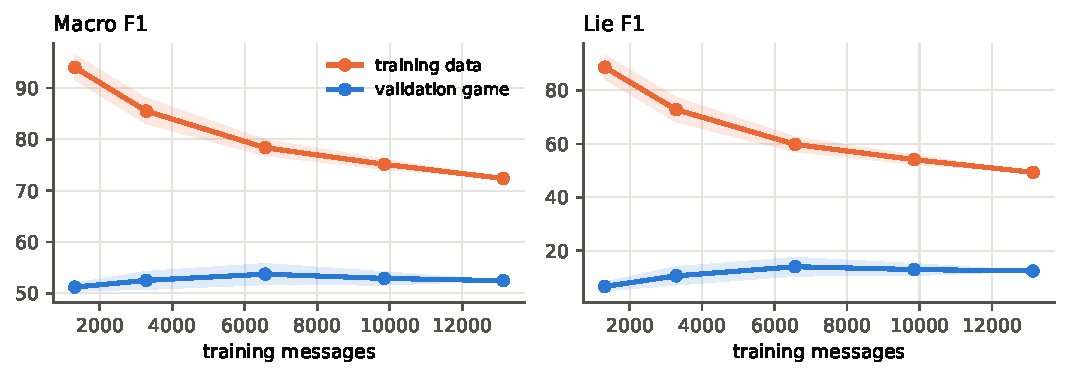
\includegraphics[width=0.8\textwidth]{fig4_learning_curve.pdf}
\caption{Learning curve of bag of words + power. Lines are means over five random samples; bands are $\pm 1$ standard deviation. The validation score stops improving after about half of the training data.}
\label{fig:lc}
\end{figure*}

\subsection{H1: do lies and truths differ in sentiment?}
\label{sec:res-h1}
Table~\ref{tab:h1} shows the Mann--Whitney tests on the 10 development games, and Fig.~\ref{fig:auc} compares the effect sizes with message length.

\begin{table}[t]
\centering
\caption{H1: lies vs.\ truths in sentiment (development games, 647 lies vs.\ 13{,}901 truths). AUC $>0.5$ means lies score higher. $p$ is Holm-corrected within each scorer.}
\label{tab:h1}
\setlength{\tabcolsep}{4pt}
\begin{tabular}{lcccc}
\toprule
Feature & Median lie & Median truth & AUC & $p_{\text{Holm}}$ \\
\midrule
VADER compound   & 0.318 & 0.197 & \best{0.547} & \best{0.0002} \\
VADER positive   & 0.134 & 0.119 & 0.522 & 0.115 \\
VADER negative   & 0.000 & 0.000 & 0.536 & \best{0.001} \\
VADER neutral    & 0.798 & 0.803 & 0.483 & 0.139 \\
\midrule
RoBERTa score    & $-0.005$ & 0.005 & 0.498 & 0.866 \\
RoBERTa positive & 0.109 & 0.093 & 0.512 & 0.866 \\
RoBERTa negative & 0.125 & 0.109 & 0.512 & 0.866 \\
RoBERTa neutral  & 0.479 & 0.539 & \best{0.462} & \best{0.005} \\
\midrule
\textit{Words per message} & \textit{20} & \textit{14} & \textit{0.618} & $3\times10^{-24}$ \\
\bottomrule
\end{tabular}
\end{table}

\begin{figure}[t]
\centering
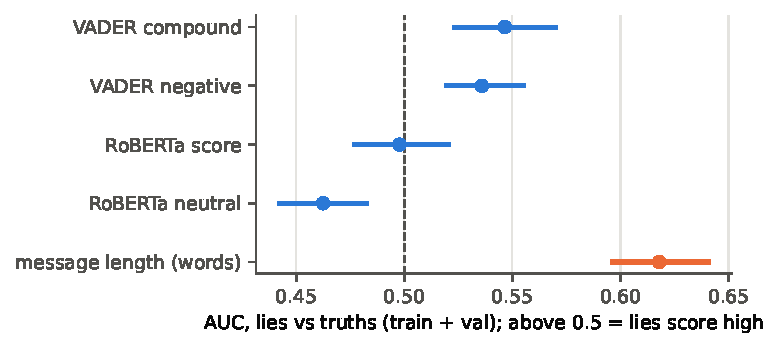
\includegraphics[width=\columnwidth]{fig2_h1_auc.pdf}
\caption{Effect sizes for H1 (AUC with 95\% bootstrap intervals). Every sentiment score is close to 0.5 (no difference). Message length (orange) separates lies from truths more strongly than any sentiment score.}
\label{fig:auc}
\end{figure}

Three findings stand out:
\begin{enumerate}
\item \textbf{The differences are statistically significant but negligible.} Lies are slightly \emph{more positive} according to VADER (compound AUC 0.547, $r = 0.093$, $p_{\text{Holm}} = 0.0002$), and the sign holds in 8 of the 10 games. They are slightly \emph{less neutral} according to RoBERTa (AUC 0.462, $r = -0.075$). RoBERTa's polarity shows no difference at all (AUC 0.498). Every effect has $|r| < 0.1$. The positive direction is in line with Niculae et al.'s finding that betrayers become more positive~\cite{niculae2015harbingers}, rather than the negative-emotion cue of laboratory studies~\cite{newman2003lying}.
\item \textbf{Length is a stronger signal than sentiment.} Lies have a median of 20 words against 14 for truths (AUC 0.618), the Pinocchio effect~\cite{vanswol2012pinocchio}. Length is correlated with VADER compound (Spearman 0.19).
\item \textbf{Most of the sentiment effect is a length effect.} Within length bins (Fig.~\ref{fig:bins}), the VADER difference disappears in the three middle bins (AUC 0.47--0.50, $p > 0.28$) and is significant only for the longest messages (32+ words: AUC 0.569, $p = 0.001$).
\end{enumerate}
The tone-change features, tested in the same way, show even smaller differences. After Holm correction over the 13 features only \texttt{has\_prev} is significant (lies are slightly more often a sender's first message to a receiver), and every $|r|$ is below 0.06.

\textbf{Verdict on H1.} Supported in the statistical sense, but the effect is too small to be useful on its own and is largely explained by message length.

\begin{figure}[t]
\centering
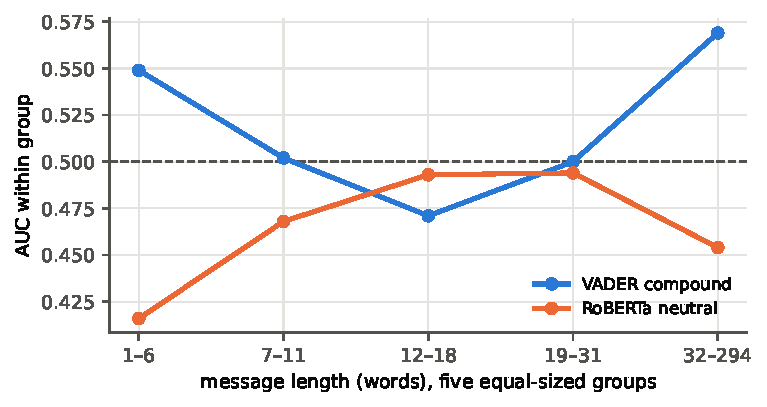
\includegraphics[width=\columnwidth]{fig3_length_bins.pdf}
\caption{H1 within five equal-sized message-length groups. Once length is held roughly fixed, the sentiment differences mostly vanish, except for the longest messages.}
\label{fig:bins}
\end{figure}

\subsection{Go / no-go decision}
\label{sec:res-go}
The plan included a checkpoint after the first experiments. The evidence showed that:
\begin{itemize}
\item the pipeline is sound, since the baselines are reproduced;
\item the task is limited by the signal, not by the amount of data;
\item the sentiment signal exists but is weak and tied up with length.
\end{itemize}
The proposal's fallback, if the signal proved too weak, was to narrow the project to a statistical analysis of sentiment in lies. Because H1 was significant and the learning curve showed the data to be sufficient for simple models, we decided to continue with the classifiers, with two changes. First, sentiment is treated as a weak, complementary signal, and a clean negative result is an acceptable outcome. Second, every sentiment model is compared against a length control, so that a gain from sentiment is not really a gain from length.

\subsection{H2: a classifier on sentiment and tone change only}
\label{sec:res-lr}
Table~\ref{tab:lr} shows the logistic regression results under LOGO (pooled out-of-game predictions) and on the test games, and Table~\ref{tab:h2} gives the paired comparisons.

\textbf{H2 itself.} The sentiment + tone-change model (S+T) beats the majority class in every one of the 10 held-out games (mean $+3.1$ macro F1, Wilcoxon $p = 0.002$). On the test games it reaches 50.3 macro F1 against 47.7, a gain of $+2.5$ with a 95\% bootstrap interval of [$+0.6$, $+4.6$] ($p = 0.004$). It therefore also clears the 47.8 threshold set in the proposal. \textbf{H2 is supported}, but the margin is small, and the comparisons with the other feature sets show what drives it.

\begin{table}[t]
\centering
\caption{Logistic regression feature sets. LOGO: pooled out-of-game predictions over the 10 development games (nested cutoff). Test: fit on all development games.}
\label{tab:lr}
\setlength{\tabcolsep}{3.5pt}
\begin{tabular}{lcccccc}
\toprule
 & \multicolumn{3}{c}{LOGO (dev)} & \multicolumn{3}{c}{Test} \\
\cmidrule(lr){2-4}\cmidrule(lr){5-7}
Features & AUC & Mac.\ F1 & Lie F1 & AUC & Mac.\ F1 & Lie F1 \\
\midrule
Majority         & 50.0 & 48.9 & \phantom{0}0.0 & 50.0 & 47.7 & \phantom{0}0.0 \\
L (length)     & 61.6 & \best{53.4} & \best{12.3} & \best{66.7} & \best{55.8} & \best{17.4} \\
S (sentiment)    & 56.1 & 52.1 & \phantom{0}8.0 & 55.1 & 51.7 & \phantom{0}9.2 \\
S+T              & 57.9 & 51.9 & \phantom{0}8.3 & 49.4 & 50.3 & \phantom{0}9.0 \\
L+S              & 61.5 & 53.2 & 11.4 & 65.1 & 53.6 & 13.4 \\
L+S+T            & \best{62.6} & 51.7 & \phantom{0}8.4 & 57.8 & 50.9 & 10.6 \\
\bottomrule
\end{tabular}
\end{table}

\begin{table}[t]
\centering
\caption{H2: paired comparisons over the 10 held-out games (mean gain, games improved, Wilcoxon signed-rank $p$). The first two rows test H2 as defined in the proposal; the others show what drives the result.}
\label{tab:h2}
\setlength{\tabcolsep}{4pt}
\begin{tabular}{llccc}
\toprule
Comparison & Metric & Gain & Games up & $p$ \\
\midrule
S+T vs.\ majority & Macro F1 & $+3.1$ & 10/10 & \best{0.002} \\
S vs.\ majority   & Macro F1 & $+2.5$ & 9/10 & \best{0.014} \\
\midrule
\multirow{2}{*}{S+T vs.\ S}     & AUC      & $+2.7$ & 8/10 & 0.23 \\
                                 & Macro F1 & $+0.6$ & 6/10 & 0.63 \\
\midrule
\multirow{2}{*}{L+S+T vs.\ L+S} & AUC      & $+3.0$ & 8/10 & \best{0.02} \\
                                 & Macro F1 & $+0.3$ & 6/10 & 0.77 \\
\midrule
\multirow{2}{*}{L+S vs.\ L}     & AUC      & $+0.3$ & 4/10 & 0.77 \\
                                 & Macro F1 & $+0.2$ & 5/10 & 1.00 \\
\bottomrule
\end{tabular}
\end{table}

\textbf{What drives it.} Three further findings qualify H2:
\begin{itemize}
\item \textbf{Sentiment adds nothing beyond length.} L+S is no better than L ($+0.3$ AUC, $p = 0.77$).
\item \textbf{Tone change improves ranking but not decisions.} With length controlled, tone change raises the AUC by 3.0 points, in 8 of 10 games ($p = 0.02$), but the macro F1 changes by only $+0.3$ ($p = 0.77$).
\item \textbf{The AUC gain does not carry over to the test games.} There, L+S+T has a lower AUC than L+S (57.8 vs.\ 65.1). The best logistic regression on test is length alone (55.8 / 17.4), which beats every model that uses sentiment and even the bag-of-words baseline in macro F1.
\end{itemize}

\textbf{Verdict on H2.} Supported: sentiment and tone change alone carry a real but weak signal, enough to beat the majority class. Most of that signal, however, is also available from message length, and tone change adds to sentiment only in ranking (AUC), not in F1.

\subsection{Fine-tuned RoBERTa: models (c), (d), (e)}
\label{sec:res-ft}
Table~\ref{tab:ft} summarises the 15 fine-tuning runs, and Fig.~\ref{fig:seeds} shows every run together with the seed ensembles.

\begin{table}[t]
\centering
\caption{Fine-tuned models, mean $\pm$ std over 5 seeds. Val AP: validation average precision (chance $\approx 4$). Test: val-chosen cutoff; @0.5: fixed cutoff.}
\label{tab:ft}
\setlength{\tabcolsep}{2.5pt}
\begin{tabular}{lccccc}
\toprule
Model & Val AP & \multicolumn{2}{c}{Test (val cutoff)} & \multicolumn{2}{c}{Test @0.5} \\
\cmidrule(lr){3-4}\cmidrule(lr){5-6}
 & & Mac.\ F1 & Lie F1 & Mac.\ F1 & Lie F1 \\
\midrule
(c) + power     & 8.0$\pm$1.3 & 54.6$\pm$2.4 & 15.2$\pm$5.1 & 48.8$\pm$4.0 & 19.1$\pm$2.6 \\
(d) + sentiment & 6.7$\pm$2.0 & 52.2$\pm$3.2 & 11.1$\pm$7.5 & 45.5$\pm$10.8 & 17.5$\pm$2.0 \\
(e) + tone      & 8.4$\pm$2.0 & 54.8$\pm$1.6 & 16.6$\pm$3.3 & 48.9$\pm$5.8 & 21.2$\pm$1.9 \\
\bottomrule
\end{tabular}
\end{table}

\begin{figure*}[t]
\centering
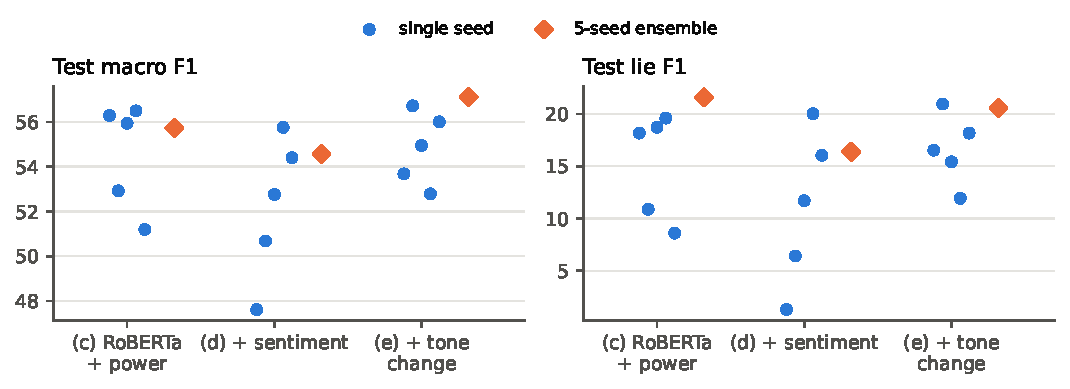
\includegraphics[width=0.8\textwidth]{fig5_seeds.pdf}
\caption{Test scores of each fine-tuning run (blue, one dot per seed) and of the five-seed ensembles (orange). The spread between seeds is as large as the differences between models; ensembling raises every model.}
\label{fig:seeds}
\end{figure*}

Three observations stand out:
\begin{itemize}
\item \textbf{Large seed variance.} The best epoch ranges from 1 to 5, the val-chosen cutoff from 0.53 to 0.97, and test macro F1 from 47.6 to 56.7. One run, (d) with seed 0, nearly collapsed (lie F1 1.3). Re-running the same configuration on the GPU changed the scores by about one F1 point, because GPU training is not bit-for-bit reproducible.
\item \textbf{Seed ensembles help.} Averaging the five seeds adds 1--2 macro F1 over the single-seed mean for every model. (e) reaches 57.1 macro F1, and (c) reaches 21.6 lie F1.
\item \textbf{The fixed 0.5 cutoff flags too many messages.} With a 0.5 cutoff, lie F1 is higher (19--21) but macro F1 drops to 45--49, because the under-sampled training makes the model over-predict lies on the natural distribution. The tuned cutoff is therefore essential.
\end{itemize}

\subsection{Main results and hypotheses H3, H4}
\label{sec:res-hyp}
Table~\ref{tab:main} and Fig.~\ref{fig:main} put all models side by side, and Table~\ref{tab:hyp} summarises the hypothesis tests against the criteria of our proposal.

\begin{table*}[t]
\centering
\caption{Main results on the test games (\textsc{Actual Lie}, 2{,}741 messages). $\pm$: std over 5 seeds. [ ]: 95\% bootstrap interval over test messages. Peskov et al.'s values are read from Fig.~5 of~\cite{peskov2020takes}.}
\label{tab:main}
\begin{tabular}{llcccc}
\toprule
Group & Model & Macro F1 & 95\% CI & Lie F1 & 95\% CI \\
\midrule
\multirow{4}{*}{Peskov et al.~\cite{peskov2020takes}}
 & Majority                      & 47.8 & & \phantom{0}0.0 & \\
 & Bag of words + power          & 54.9 & & 20.2 & \\
 & Context LSTM + power (best)   & 57.2 & & \best{27.0} & \\
 & Human receivers               & 58.1 & & 22.5 & \\
\midrule
\multirow{3}{*}{Our baselines}
 & Majority                      & 47.7 & & \phantom{0}0.0 & \\
 & Bag of words + power          & 54.7 & & 19.8 & \\
 & Human receivers (recomputed)  & 58.1 & & 22.5 & \\
\midrule
\multirow{4}{*}{Logistic regression}
 & L: length only                & 55.8 & & 17.4 & \\
 & S: sentiment                  & 51.7 & & \phantom{0}9.2 & \\
 & S+T: sentiment + tone change  & 50.3 & & \phantom{0}9.0 & \\
 & L+S+T                         & 50.9 & & 10.6 & \\
\midrule
\multirow{6}{*}{Fine-tuned RoBERTa}
 & (c) + power, single seed            & 54.6$\pm$2.4 & & 15.2$\pm$5.1 & \\
 & (d) + sentiment, single seed        & 52.2$\pm$3.2 & & 11.1$\pm$7.5 & \\
 & (e) + tone change, single seed      & 54.8$\pm$1.6 & & 16.6$\pm$3.3 & \\
 & (c) + power, 5-seed ensemble        & 55.7 & [53.5, 58.0] & 21.6 & [17.6, 25.7] \\
 & (d) + sentiment, 5-seed ensemble    & 54.6 & [52.2, 57.0] & 16.4 & [11.9, 21.0] \\
 & (e) + tone change, 5-seed ensemble  & \best{57.1} & [54.4, 59.8] & 20.6 & [15.5, 25.8] \\
\bottomrule
\end{tabular}
\end{table*}

\begin{figure*}[t]
\centering
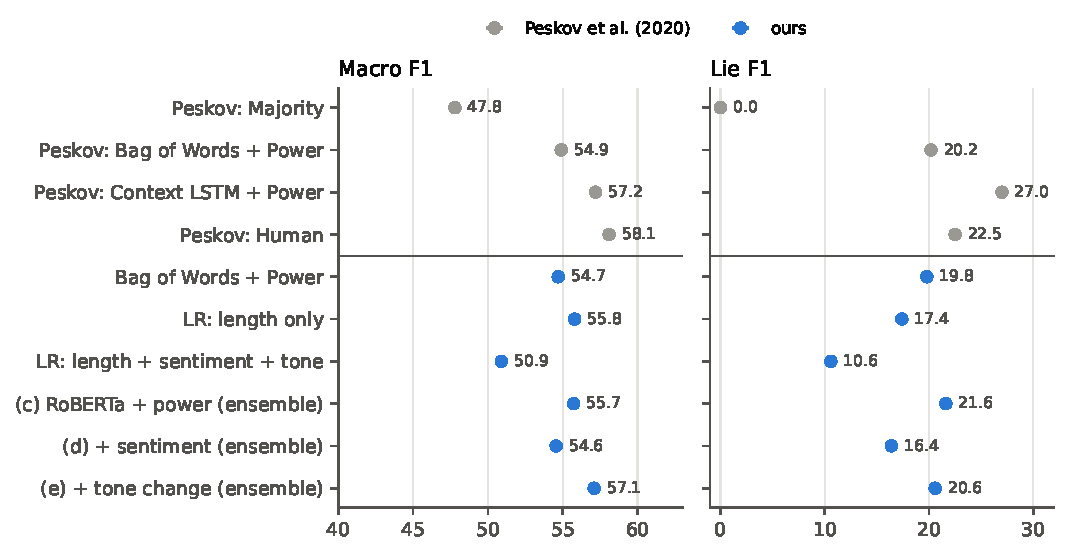
\includegraphics[width=0.9\textwidth]{fig1_results.pdf}
\caption{Test results compared with Peskov et al.\ (grey). Error bars on our fine-tuned models are $\pm 1$ std over five seeds. Our best macro F1 (the (e) ensemble, 57.1) is within 0.1 of Peskov's best model, but every model of ours remains well below its lie F1 of 27.0.}
\label{fig:main}
\end{figure*}

\begin{table}[t]
\centering
\caption{Hypotheses as defined in the proposal. Seeds: mean paired difference over 5 seeds (seeds improved). Ens.: five-seed ensembles, gain [95\% CI], one-sided paired-bootstrap $p$.}
\label{tab:hyp}
\setlength{\tabcolsep}{3pt}
\renewcommand{\arraystretch}{1.1}
\begin{tabular}{>{\raggedright\arraybackslash}p{1.55cm}>{\raggedright\arraybackslash}p{3.45cm}>{\raggedright\arraybackslash}p{2.3cm}}
\toprule
Hypothesis (criterion) & Evidence & Verdict \\
\midrule
H1 sentiment differs ($p<0.05$) & VADER compound: AUC 0.547, $p_{\text{Holm}}{=}0.0002$; RoBERTa neutral: AUC 0.462, $p_{\text{Holm}}{=}0.005$ & \textbf{Supported}, but negligible ($|r|<0.1$) and mostly length \\
\midrule
H2 S+T beats majority (macro F1 $>47.8$) & Test 50.3 vs.\ 47.7: $+2.5$ [$+0.6$, $+4.6$]; LOGO: 10/10 games, $p{=}0.002$ & \textbf{Supported}; length alone does better (55.8) \\
\midrule
H3 (d) vs.\ (c) (lie F1 $\ge +1$) & Seeds: $-4.1$ (2/5); ens.: $-5.2$ [$-9.4$, $-1.2$] & \textbf{Not supported}; sentiment \emph{hurts} \\
\midrule
H4 (e) vs.\ (d) (lie F1 $\ge +1$) & Seeds: $+5.5$ (4/5); ens.: $+4.2$ [$+0.1$, $+8.3$], $p{=}0.02$ & \textbf{Supported}; mostly recovers H3's loss \\
\midrule
\textit{(e) vs.\ (c), both additions} & Lie F1: seeds $+1.4$ (2/5), ens.\ $-1.0$; macro F1: ens.\ $+1.4$ [$-0.8$, $+3.3$], $p{=}0.09$ & No reliable gain \\
\bottomrule
\end{tabular}
\end{table}

\begin{table}[t]
\centering
\caption{Success criteria from the proposal (test, macro F1 / lie F1) and what we achieved.}
\label{tab:criteria}
\setlength{\tabcolsep}{3pt}
\begin{tabular}{lccc}
\toprule
Criterion & Required & Achieved & Met \\
\midrule
Sentiment-only (H2)     & $>47.8$ / -- & 50.3 / \phantom{0}9.0 & $\checkmark$ \\
Full model, minimum     & $>57.2$ / $>22.5$ & & \\
\quad mean of 5 seeds   & & 54.8 / 16.6 & $\times$ \\
\quad 5-seed ensemble   & & 57.1 / 20.6 & $\times$ \\
Full model, target      & $>58.1$ / $>27.0$ & 57.1 / 20.6 & $\times$ \\
\bottomrule
\end{tabular}
\end{table}

\begin{itemize}
\item \textbf{Best model.} The (e) ensemble reaches 57.1 / 20.6. Its macro F1 is within 0.1 of Peskov et al.'s best model (57.2) with a much simpler architecture, but its lie F1 is clearly lower (27.0). Its 95\% interval [54.4, 59.8] still includes the bag-of-words baseline (54.7), so it is not clearly better than bag of words.
\item \textbf{H3 is not supported: sentiment features hurt.} Adding the 8 sentiment scores to (c) lowers lie F1 by 4.1 points on average over the seeds (the criterion was a gain of at least 1), lowers macro F1 in 4 of 5 seeds, and lowers the ensemble's lie F1 by 5.2 points, an interval that excludes zero. A likely reason is that the fine-tuned encoder already represents the sentiment of the text, so the scores add little new information and some noise, and they increase the risk of overfitting a very small set of lies.
\item \textbf{H4 is supported, but mainly recovers H3's loss.} Tone change raises lie F1 over (d) by 5.5 points on average, in 4 of 5 seeds, and by 4.2 on the ensembles ($p = 0.02$). Compared with (c), however, the full model gains only $+1.4$ lie F1 on average (better in 2 of 5 seeds), and its ensemble is 1.0 lie F1 \emph{lower} than (c)'s.
\item \textbf{Success criteria (Table~\ref{tab:criteria}).} The sentiment-only criterion is met. The full model does not reach the minimum: its ensemble falls 0.1 macro F1 and 1.9 lie F1 short, and the mean over seeds falls further short.
\end{itemize}

\subsection{Error analysis}
\label{sec:res-err}
We analyse the (e) ensemble on the test games, with (c) for comparison.

\textbf{Few, often wrong flags.} The model flags 168 of the 2,741 messages. Of these, 42 are lies (precision 25.0\%), and they cover 17.5\% of the 240 lies.

\textbf{One game carries the score.} Game 4 (1,546 messages, 12.5\% lies) scores 57.2 / 23.6, while game 12 (1,195 messages, only 3.9\% lies) scores 52.4 / 7.8. With two test games, the headline number depends heavily on which games happen to be in the test set.

\textbf{The model behaves like a ``long message'' detector} (Fig.~\ref{fig:err}):
\begin{itemize}
\item It finds none of the lies of 6 words or fewer and 36\% of those with 32 or more words.
\item Caught lies have a median length of 50.5 words, against 21 for missed lies.
\item False alarms are long too: a median of 34 words, against 12 for correctly passed truths.
\item Caught lies and false alarms also have higher VADER compound scores (medians 0.60 and 0.49) than missed lies and correct truths (0.25 and 0.10), simply because longer messages contain more sentiment words.
\end{itemize}

\begin{figure}[t]
\centering
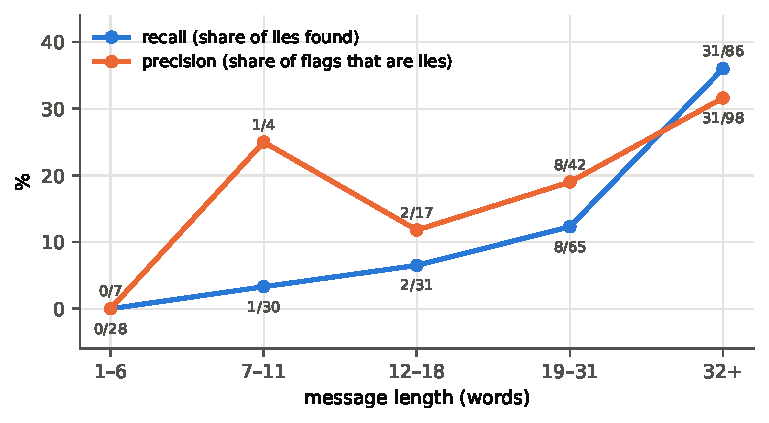
\includegraphics[width=\columnwidth]{fig6_errors_by_length.pdf}
\caption{Error analysis of the (e) ensemble by message length. Labels give counts: caught/lies (recall) and caught/flagged (precision). Short lies are never caught.}
\label{fig:err}
\end{figure}

\textbf{Power.} Senders more than four supply centres ahead lie most often (15.3\% of their messages), but the model finds only 2 of their 23 lies.

\textbf{Comparison with humans.} Table~\ref{tab:human} conditions on lies that have a receiver label, as in Table~5 of Peskov et al. Our table is almost identical to theirs. Two thirds of all lies fool both the model and the receiver, and the two catch largely \emph{different} lies: only 10 lies are caught by both. This suggests that combining human and model judgements could help.

\begin{table}[t]
\centering
\caption{Model vs.\ human receivers on the 207 test lies with a receiver label. Ours: (e) ensemble; in brackets, Peskov et al.'s Context LSTM + power (their Table~5).}
\label{tab:human}
\begin{tabular}{lcc}
\toprule
 & Model caught & Model missed \\
\midrule
Receiver caught & 10 (10) & \phantom{0}32 (32) \\
Receiver fooled & 27 (28) & 138 (137) \\
\bottomrule
\end{tabular}
\end{table}

\textbf{(e) vs.\ (c).} Every lie that (e) catches is also caught by (c). The higher macro F1 of (e) comes from flagging far fewer messages (168 vs.\ 389, due to a higher val-chosen cutoff), not from finding new lies.

\textbf{Examples.} The most confident false alarms are long, emotional messages about alliances or strategy (``Your basically for sure my ally now. Early in the game I was debating an alliance with Austria\dots''). The lies the model is most sure are true are short and concrete: ``Sorry for the all the messages'', ``Damn! I changed my orders but they didn't go through for some reason''. Peskov et al.\ also found this kind of terse lie the hardest to catch.

% =====================================================================
\section{Discussion and Limitations}
\label{sec:discussion}

\textbf{Sentiment is mostly a proxy for length.} The same confound appears in every experiment:
\begin{itemize}
\item in H1, where the sentiment differences mostly vanish within length bins;
\item in H2, where sentiment adds nothing on top of length;
\item in the error analysis, where the fine-tuned model's catches and false alarms are both long and both positive.
\end{itemize}
A length-only logistic regression is a surprisingly strong baseline (55.8 macro F1), and we recommend that future work on this dataset report it.

\textbf{Small evaluation sets.} The validation split has 56 lies and the test split two games. Selecting the epoch and cutoff on one validation game is noisy, which shows in the seed variance, and the test score is dominated by game 4. Our bootstrap intervals assume independent messages and are therefore optimistic.

\textbf{Comparability.} Peskov et al.'s numbers are read from a bar chart, and some may be computed on the 2,475 receiver-labelled test messages rather than all 2,741. Both effects are below 0.3 F1 for the baselines we could check. Two choices differ from our proposal. The fine-tuned models use under-sampling together with the class-weighted loss, because the planned class-weighted setup alone did not train, and model (c) includes the power features (Section~\ref{sec:design-ft}).

% =====================================================================
\section{Conclusion and Next Steps}
\label{sec:conclusion}

\subsection{Summary of work and results}
We built a reproducible pipeline for lie detection on the \textit{Diplomacy} dataset and used it to test whether sentiment and tone change help. The main results are:
\begin{itemize}
\item The bag-of-words and human baselines of Peskov et al.\ are reproduced to within 0.3 macro F1.
\item \textbf{H1 supported, but weak:} lies and truths differ significantly in sentiment, but the effect is negligible and largely due to lies being longer.
\item \textbf{H2 supported:} a classifier on sentiment and tone change alone beats the majority class (50.3 vs.\ 47.7 macro F1 on test), but a classifier on message length alone does better (55.8).
\item \textbf{H3 not supported:} in a fine-tuned RoBERTa model with conversational context and power, sentiment features lower lie F1 by 4.1 points on average.
\item \textbf{H4 supported:} tone-change features then raise lie F1 by 5.5 points, but this mostly recovers H3's loss; the full model is not reliably better than the model with neither.
\item \textbf{Success criteria not yet met:} our best model, a five-seed ensemble of the full model, reaches 57.1 macro F1 and 20.6 lie F1, just short of the proposal's minimum (57.2 / 22.5) and well below Peskov et al.'s lie F1 (27.0).
\end{itemize}
So far, then, the answer to our research question is \emph{largely negative}: on this dataset, explicit sentiment and tone-change features do not reliably improve lie detection beyond what message length and the text itself provide.

\subsection{Steps to be taken from now on}
\begin{enumerate}
\item \textbf{Remove the length confound from the evaluation.} Add message length explicitly to the fine-tuned models' feature vector, so that (c)--(e) all share the same length control as the logistic regressions. Also report results within length bins and on a length-matched subsample of lies and truths.
\item \textbf{More robust model selection.} Choose the cutoff (and possibly the epoch) from out-of-game predictions of the seed ensemble rather than from the single validation game. If compute allows, run a reduced LOGO for the best model, to test whether the H3 and H4 conclusions hold across games and not only on the two test games.
\item \textbf{Relative and two-sided tone change.} Our tone-change features compare a sender only with themselves. Niculae et al.\ found that betrayal is foreshadowed by \emph{imbalances} between partners~\cite{niculae2015harbingers}, so we will add features that compare the sender's tone with the receiver's recent tone.
\item \textbf{Politeness features} (optional in our plan). Politeness strategies~\cite{danescu2013politeness} were another harbinger of betrayal, and would test whether a social signal other than sentiment helps where sentiment did not.
\item \textbf{Final report.} Write up the final results with the figures and tables of this report, including a qualitative analysis of the examples and a discussion of the negative result.
\end{enumerate}

% =====================================================================
\bibliographystyle{IEEEtran}
\bibliography{references}

\end{document}
